\documentclass{homework}

%% Import a package useful for displaying graphics.
\usepackage{graphicx}

%% Feel free to add your own commonly used commands to this file.

\newcommand{\Reals}{\ensuremath{\mathbb R}}% Gives you a shortcut for writing the blackboard R for the real numbers - \RR
\newcommand{\Nats}{\ensuremath{\mathbb N}} % Gives you a shortcut for writing the blackboard N for the natural numbers - \NN
\newcommand{\Ints}{\ensuremath{\mathbb Z}} % Gives you a shortcut for writing the blackboard Z for the integer numbers - \ZZ
\newcommand{\Rats}{\ensuremath{\mathbb Q}} % Gives you a shortcut for writing the blackboard Q for the rational numbers - \QQ
\newcommand{\Cplx}{\ensuremath{\mathbb C}} % Gives you a shortcut for writing the blackboard C for the complex numbers - \CC

% Make better absolute value bars and the norm symbol
\newcommand{\abs}[1]{\left|#1\right|}
\newcommand{\norm}[1]{\left|\left|\,#1\,\right|\right|}


% The following commands set up the material that appears
% in the header.
\doclabel{Math 490: Demo Homework}
\docauthor{Your name here.}
\docdate{January 12, 2019}

\begin{document}
\begin{problems}

\problem 
If $a$ and $b$ are even integers, then so is $a+b$.
\solution
Let $a$ and $b$ be even integers.  Then there exist integers
$j$ and $k$ such that $a=2j$ and $b=2k$.  But then
\begin{equation}
a+b = 2j+ 2k = 2(j+k).
\end{equation}
Since $j+k\in\Ints$, $a+b$ is even.


\problem
Plot $\sin(x)$ and $\cos(x)$ for $-\pi \le x \le \pi$ on the same graph.
Make sure the graph is labeled nicely.
\solution
\begin{verbatim}
octave:1> x=[-pi:0.01:pi];
octave:2> plot(x,sin(x),x,cos(x));
octave:3> set(gca, "fontsize", 14 )
octave:4> xlabel("x");ylabel("y");title("sin and cos");
octave:5> legend("sin","cos");
\end{verbatim}
\begin{center}
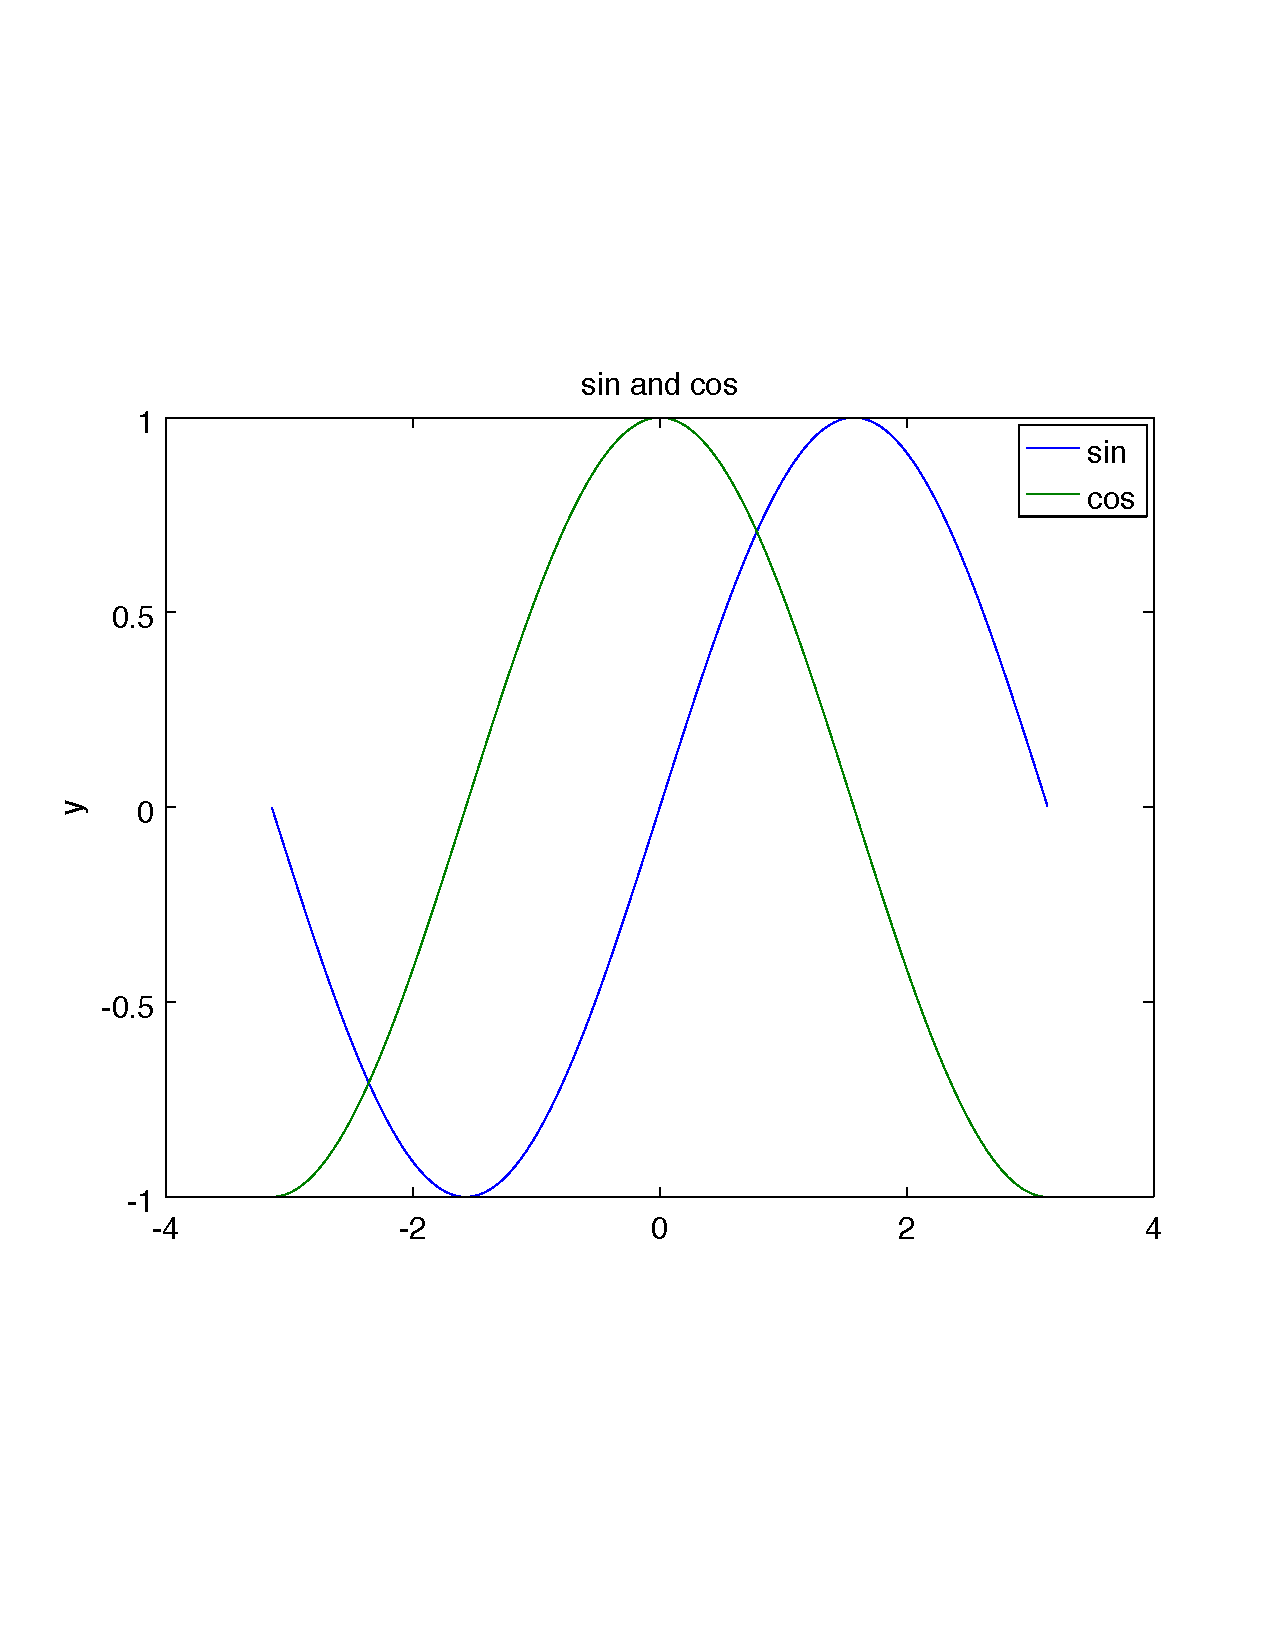
\includegraphics[width=5in]{prob2.pdf}
\end{center}

\end{problems}
\end{document}